\documentclass{article}
\usepackage{neurips_data_2024}
\usepackage[utf8]{inputenc} % allow utf-8 input
\usepackage[T1]{fontenc}    % use 8-bit T1 fonts
\usepackage{hyperref}       % hyperlinks
\usepackage{url}            % simple URL typesetting
\usepackage{booktabs}       % professional-quality tables
\usepackage{amsfonts}       % blackboard math symbols
\usepackage{nicefrac}       % compact symbols for 1/2, etc.
\usepackage{microtype}      % microtypography
\usepackage{xcolor}         % colors
\usepackage{lipsum}
\usepackage{graphicx}       % include pdfs as figures

\title{\texttt{metabench}\\A Sparse Benchmark to Measure General Ability\\in Large Language Models}
\author{%
   Alex Kipnis $^{1}$ \thanks{Correspondence to \texttt{adkipnis@mailbox.org}} \quad
   Luca M. Schulze Buschoff $^{1}$ \quad
   Konstantinos Voudouris $^{1,2}$ \quad
   Eric Schulz $^1$\\
   $^1$ Human-Centered AI, Helmholtz Munich \quad $^2$ University of Cambridge\\
}

\begin{document}

\maketitle

\begin{abstract}
   Large Language Models (LLMs) vary in their abilities on a range of tasks. Initiatives such as the \texttt{Open LLM Leaderboard} aim to quantify these differences with several large benchmarks (sets of test items to which an LLM can respond either correctly or incorrectly).
   However, high correlations within and between benchmark scores suggest that (1) there exists a small set of common underlying abilities that these benchmarks measure, and (2) the latter tap into redundant information and may thus be considerably compressed.
   We use data from over $4.000$ LLMs to analyze the psychometric properties of six benchmarks (\texttt{ARC}, \texttt{GSM8K}, \texttt{HellaSwag}, \texttt{MMLU}, \texttt{TruthfulQA} and \texttt{WinoGrande}) in order to identify their most informative items.
   Using this subset, we construct a sparse benchmark, \texttt{metabench}, that has less than $4$\% of the original size of all six benchmarks combined. Moreover, \texttt{metabench} goes beyond point scores by yielding estimators of the underlying benchmark-specific abilities.
   We show that these estimators (1) can be used to reconstruct the original \textit{individual} benchmark scores, and (2) have one underlying common factor which can be used to reconstruct the original \textit{total} score with $\sim 2$\% error.
\end{abstract}

\section{Introduction}
% add figure (overview.pdf) here
% begin figure
\begin{figure}[h]
   \centering
   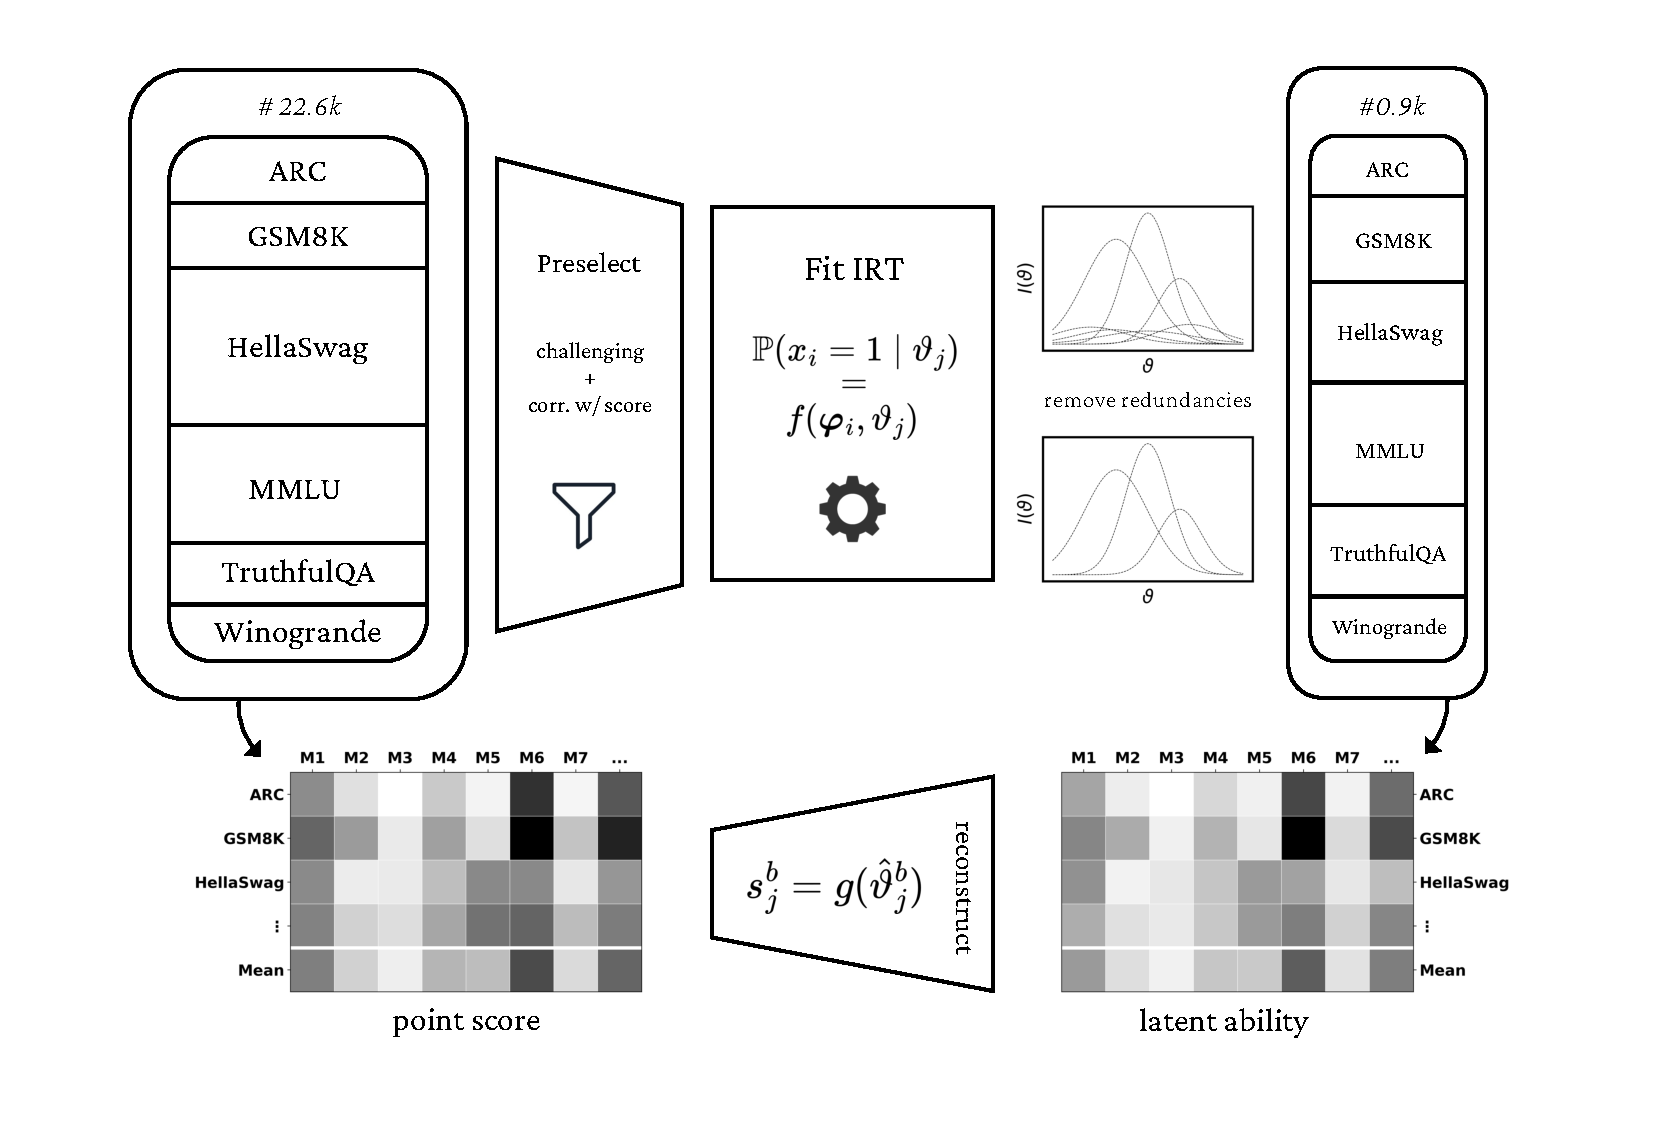
\includegraphics[width=0.8\textwidth]{figures/overview.pdf}
   \caption{\textit{Processing pipeline}. (1) Collect item-wise accuracies from all available LLMs for each benchmark on \texttt{Open LLM Leaderboard}. (2) Remove items solved by more than $95\%$ of LLMs and items with part-whole correlation $r \approx 0$. (3) Fit variants of IRT models to the remaining items and choose the best fit by cross-validation. (4) Infer item information from the item parameters and filter out uninformative items to (5) construct \texttt{metabench}. (6) Use the item parameters to estimate the benchmark-specific abilities and use factor analysis to find a common factor. (7) These can be used to reconstruct the original (normalized) benchmark scores as well as their mean.}
   \label{fig:overview}
\end{figure}


\subsection{Related Work}
\section{Psychometric Analysis}
\section{Benchmark Distillation}
\section{Going Beyond Points}
\section{Conclusion}
\subsection{Limitations}
\section{Future Work}
\section*{Acknowledgments}
\section*{References}
\end{document}
